%%%%%%%%%%%%%%%%%%%%%%%%%%%%%%%%%%%%%%%%%
% Beamer Presentation
% LaTeX Template
% Version 1.0 (10/11/12)
%
% This template has been downloaded from:
% http://www.LaTeXTemplates.com
%
% License:
% CC BY-NC-SA 3.0 (http://creativecommons.org/licenses/by-nc-sa/3.0/)
%
%%%%%%%%%%%%%%%%%%%%%%%%%%%%%%%%%%%%%%%%%

%----------------------------------------------------------------------------------------
%	PACKAGES AND THEMES
%----------------------------------------------------------------------------------------

\documentclass[aspectratio=169,UTF8,11pt,t]{ctexbeamer}

\mode<presentation> {
	\usetheme{Madrid}
	\setbeamertemplate{footline}{} % To remove the footer line in all slides
	\setbeamertemplate{navigation symbols}{} % To remove the navigation symbols from the bottom of all slides
}

% User Defined Block %%%%%%%%%%%%%%%%%%%%%%%%%%%%%%%%%%%%%%%%%%%%%%%%%%%%%%%%
\usepackage{multirow}

\usepackage{setspace}
\definecolor{hanblue}{rgb}{0.27, 0.42, 0.81}
\definecolor{indiagreen}{rgb}{0.07, 0.53, 0.03}
\definecolor{indianred}{rgb}{0.8, 0.36, 0.36}
\definecolor{indianyellow}{rgb}{0.89, 0.66, 0.34}
\definecolor{babypink}{rgb}{0.96, 0.76, 0.76}
\definecolor{ao(english)}{rgb}{0.0, 0.5, 0.0}
%\setbeamerfont{block title}{size=\small}
%\setbeamerfont{block body}{size=\footnotesize}
\newenvironment<>{blueblock}[1]{%
	\setbeamercolor{block title}{fg=white,bg=hanblue}%
	\begin{block}#2{#1}}{\end{block}}
\newenvironment<>{greenblock}[1]{%
	\setstretch{1.3}\setbeamercolor{block title}{fg=white,bg=indiagreen}%
	\begin{block}#2{#1}}{\end{block}}
\newenvironment<>{redblock}[1]{%
	\setstretch{1.3}\setbeamercolor{block title}{fg=white,bg=indianred}%
	\begin{block}#2{#1}}{\end{block}}
\newenvironment<>{yellowblock}[1]{%
	\setstretch{1.3}\setbeamercolor{block title}{fg=white,bg=indianyellow}%
	\begin{block}#2{#1}}{\end{block}}

%----------------------------------------------------------------------------------------
%	PACKAGES
%----------------------------------------------------------------------------------------
\usepackage{graphicx} % Allows including images
%\usepackage{tikz}
%\usetikzlibrary{shapes.geometric, arrows}
\usepackage{listings}
\lstset{language=C++,
	columns=flexible,
	basicstyle=\small\ttfamily,                                      % 设定代码字体、大小
	%numbers=left,xleftmargin=2em,framexleftmargin=2em,                   % 在左侧显示行号
	%numberstyle=\color{darkgray},                                        % 设定行号格式
	keywordstyle=\color{blue},                                            % 设定关键字格式
	commentstyle=\color{ao(english)},                                     % 设置代码注释的格式
	stringstyle=\color{brown},                                            % 设置字符串格式
	%showstringspaces=false,                                              % 控制是否显示空格
	%frame=lines,                                                         % 控制外框
	breaklines,                                                           % 控制是否折行
	postbreak=\space,                                                     % 控制折行后显示的标识字符
	breakindent=5pt,                                                      % 控制折行后缩进数量
	emph={size\_t,array,deque,list,map,queue,set,stack,vector,string,pair,tuple,ifstream,ostream}, % 非内置类型
	emphstyle={\color{teal}},
	escapeinside={(*@}{@*)},
}

%----------------------------------------------------------------------------------------
%	TITLE PAGE
%----------------------------------------------------------------------------------------

\title[\textit{C++程序设计:第十章}]{第十章~简单输入输出} % The short title appears at the bottom of every slide, the full title is only on the title page

%\author[李长河]{李长河} % Your name
%\institute[CUG] % Your institution as it will appear on the bottom of every slide, may be shorthand to save space
%{
%中国地质大学(武汉)\\ % Your institution for the title page
%\medskip
%\textit{lichanghe@cug.edu.cn} % Your email address
%}
\date{} % Date, can be changed to a custom date

\begin{document}
	
	%----------------------------------------------------------------------------------------
	%	TIKZ FLOWCHART
	%----------------------------------------------------------------------------------------
	%\tikzstyle{startstop} = [rectangle, rounded corners, minimum width=2cm, minimum height=0.5cm, text centered, draw=black, fill=red!30, font=\tiny]
	%\tikzstyle{io} = [trapezium, trapezium left angle=70, trapezium right angle=110, minimum width=0cm, minimum height=0cm, text centered, draw=black, fill=blue!30, font=\tiny]
	%\tikzstyle{process} = [rectangle, minimum width=2.5cm, minimum height=1.5cm, text centered, draw=black, fill=orange!30, font=\tiny, text width=2cm]
	%\tikzstyle{decision} = [diamond, minimum width=2.5cm, minimum height=2cm, text centered, draw=black, fill=green!30, font=\tiny, text width=1.8cm, aspect=1.1]
	
	\begin{frame}
		\titlepage % Print the title page as the first slide
	\end{frame}
	
	\begin{frame}{目录}
		\tableofcontents
	\end{frame}
	
	%----------------------------------------------------------------------------------------
	%	PRESENTATION SLIDES
	%----------------------------------------------------------------------------------------
	
	%--------------------
	
	\begin{frame}[fragile]{~} % Table of contents slide, comment this block out to remove it
		
		\begin{block}{学习目标}
			\begin{enumerate}
				\item 了解常用~IO~类的继承关系和理解~IO~流基本工作流程;
				\vspace{3ex}
				\item 掌握常见的输入输出格式控制;
				\vspace{3ex}
				\item 掌握文件流和~string~流的使用方法。
			\end{enumerate}
		\end{block}
		
		% ------功能模块说明,请注释掉-------
%		\begin{columns}[t]
%			\column{0.15\textwidth}
%			\begin{block}{概念}
%			\end{block}
%			\column{0.15\textwidth}
%			\begin{blueblock}{代码}
%			\end{blueblock}
%			\column{0.15\textwidth}
%			\begin{yellowblock}{说明}
%			\end{yellowblock}
%			\column{0.15\textwidth}
%			\begin{greenblock}{问题/答案}
%			\end{greenblock}
%			\column{0.15\textwidth}
%			\begin{redblock}{注意}
%			\end{redblock}
%		\end{columns}
		% ------功能模块说明,请注释掉-------
		
	\end{frame}
	
	%--------------------
	
	%#####################################
	\section{基本知识}
	%#####################################
	
	\begin{frame}[fragile]{10.1~基本知识}
		
		\begin{block}{C++的IO操作}
			\vspace{2ex}
			\begin{itemize}
				\item C++~不能直接处理~IO~操作,依靠不同的~IO~类来实现从设备中读取数据和向设备写入数据。\\
			\end{itemize}
		\end{block}
	\vspace{4ex}
		\begin{block}{例如:}
			\begin{lstlisting}
cin >> a;
cout << a << endl;
            \end{lstlisting}
		\end{block}
		

		
	\end{frame}
	
	%-------------------------------------
	\subsection{~IO~类对象}
	%-------------------------------------
	
	\begin{frame}[fragile]{10.1.1~IO~类对象}
		\begin{block}{}
		\alert{流(stream)}: 数据从数据源到目的端的流动过程。
		\end{block}
		\begin{block}{~IO~类关系}
			\begin{center}
			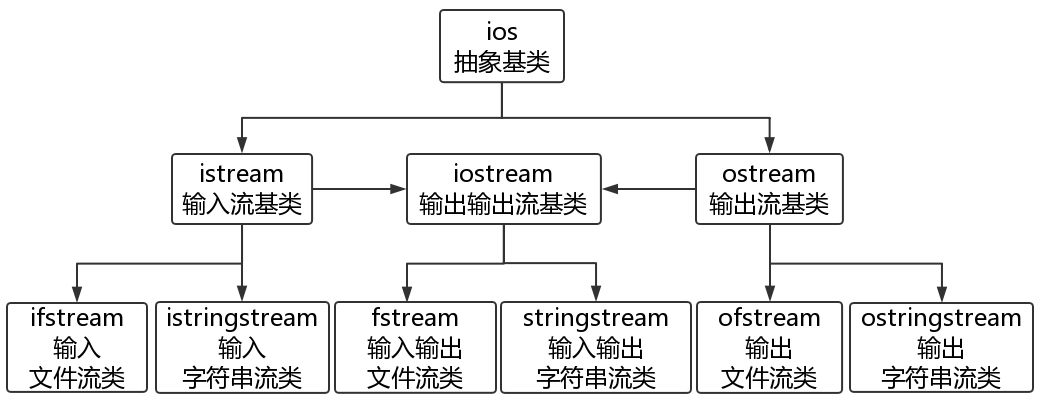
\includegraphics[width=0.95\textwidth]{fig2}
		\end{center}
		\end{block}
	\end{frame}

%	\begin{frame}[fragile]{10.1.1~IO~类对象}
%	常用IO类关系:
%	\begin{table}[t]
%		\begin{center}\ttfamily
%			\color{hanblue}\color{hanblue}\label{tab10-1}\color{hanblue}
%			\begin{tabular}{llp{0.6\textwidth}}\hline
%				头文件                    & 类名          & 功能                                 \\\hline
%				iostream                  & ios           & 抽象基类                             \\\hline
%				\multirow{3}{*}{iostream} & istream       & 通用输入流和其他输入流的基类         \\
%				& ostream       & 通用输出流和其他输出流的基类         \\
%				& iostream      & 通用输入输出流和其他输入输出流的基类 \\\hline
%				\multirow{3}{*}{fstream} & ifstream      & 输入文件流类                         \\
%				& ofstream      & 输出文件流类                         \\
%				&fstream& 输入输出文件流类                     \\\hline
%				\multirow{3}{*}{sstream}  & istringstream & 输入字符串流类                       \\
%				& ostringstream & 输出字符串流类                       \\
%				& stringstream  & 输入输出字符串流类                   \\\hline
%			\end{tabular}
%		\end{center}
%	\end{table}
%	
%	\end{frame}
	\begin{frame}[fragile]{10.1.1~IO~类对象}
		\begin{blueblock}{输入输出过程是怎样的?}
			\begin{itemize}
				\item cin~是~istream~对象,通过$>>$将内存中的输入缓冲区数据读取到与对象相关联的内存。
			\end{itemize}
		\end{blueblock}
		\begin{blueblock}<2->{数据输入的过程:}
			\begin{center}
				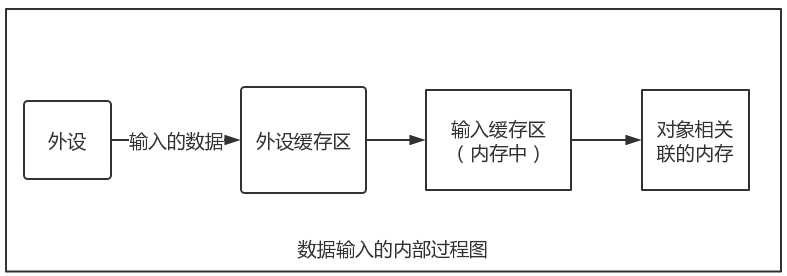
\includegraphics[width=0.8\textwidth]{fig1}
			\end{center}
		\end{blueblock}
	\end{frame}
	
%	\begin{frame}[fragile]{10.1.1~IO~类对象}
%		\begin{block}{常用对象~cin~,~cout~:}
%			\begin{itemize}
%				\item cin~是~istream~类的对象,它从标准输入设备(键盘)获取数据,通过输入运算符~\verb;>>; 。
%				
%				\item cin\verb;>>;~从流中提取数据时通常跳过输入流中的\alert{空格、制表符、换行符等空白字符}。
%				\item cout~是~ostream~类对象,它向控制台窗口输出数据。
%			\end{itemize}
%		\end{block}


	
%	\end{frame}
	
	\begin{frame}[fragile]{10.1.1~IO~类对象}
		\begin{redblock}{~IO~和普通对象的区别:}
			和普通对象不同,IO~对象不支持赋值和复制操作。
		\end{redblock}
		\begin{blueblock}{示例:}<2->
			\begin{lstlisting}[moreemph={Array}]
ifstream in1, in2;      //定义两个文件输入流对象
in1 = in2;              //错误:不能对流对象赋值

//同样,IO对象也不支持复制操作:
ostream print(ostream); //错误:不能按值方式返回或传递ostream对象
            \end{lstlisting}
		\end{blueblock}
	\end{frame}
	%-------------------------------------
	\subsection{条件状态}
	\begin{frame}[fragile]{10.1.2条件状态}
		\begin{blueblock}{请看如下情况:}\vspace{-2mm}
			\begin{lstlisting}[moreemph={Array,T,Less,F}]
double x;
cin >> x;
            \end{lstlisting}\vspace{-2mm}
		\end{blueblock}
		\begin{greenblock}{}
			当输入一个~char~类型的时候,程序会如何?
		\end{greenblock}
		\begin{greenblock}<2->{}
		当输入一个~char~类型的时候,cin~会进入错误状态,它就变成无效的,无法再执行后续的输入。因此,在使用~cin~时,要确保它的状态是有效的。
		\end{greenblock}
		\begin{blueblock}{有效性判断:}<3->\vspace{-2mm}
		\begin{lstlisting}[moreemph={Array,T,Less,F}]
while(cin >> x)     //遇到错误状态循环将退出;

if(!cin)
   cin.clear();     //clear()函数执行后,cin变为有效状态;
        \end{lstlisting}
		\vspace{-2mm}
	\end{blueblock}

	\end{frame}

	\subsection{刷新缓冲区}
	\begin{frame}[fragile]{10.1.3刷新缓冲区}
		\begin{blueblock}{缓冲区刷新:}
		导致缓冲区刷新有很多原因,比如\alert{缓冲区满、程序正常结束、遇到~endl~等}。缓冲区刷新完成后,原来的数据被清空。
		\end{blueblock}
	\vspace{4ex}
		\begin{blueblock}{示例:}
		\begin{lstlisting}[moreemph={Array,T,Less,F}]
cout << "endl" << endl;         //输出endl和一个换行,然后刷新缓冲区
cout << "flush" << flush;       //输出flush(无额外字符),然后刷新缓冲区
cout << "ends" << ends;         //输出ends和一个空字符,然后刷新缓冲区
        \end{lstlisting}
		\end{blueblock}
	\end{frame}
	
	\section{标准输入输出}
	
%	\begin{frame}[fragile]{10.2~标准输入输出}
%		输入输出的控制是C++程序当中最常用的一些操作,字符数据的格式化控制尤为重要。
%	\end{frame}
	\subsection{字符数据的输入}
	\begin{frame}[fragile]{10.2.1~字符数据的输入}
		\begin{blueblock}{\texttt{cin>>}:}<1->
			数据的输入以空白字符结束(\alert{包括空格符、制表符和回车符}等),而这些空白字符会被系统过滤掉。
		\end{blueblock}
		\vspace{4ex}
		\begin{blueblock}{cin.get():}<2->
			cin.get()~可以从输入流中获取一个字符,并将其返回。
		\end{blueblock}
	
		\begin{blueblock}{示例:}<2->
            \begin{lstlisting}[moreemph={Array,T,Less,F}]
for(char c;(c=cin.get())!='\n';)
    cout << c;
cout << endl;
            \end{lstlisting}
		\end{blueblock}

	\end{frame}
	
	\begin{frame}[fragile]{10.2.1~字符数据的输入}
		\begin{blueblock}{cin.getline():}
			getline~函数以\alert{回车符}作为输入结束的标志符,把从输入流~cin~中提取的字符序列(不包括回车符)放到~string~类对象~s~中,并返回~cin~的引用。
		\end{blueblock}
		\vspace{4ex}
		\begin{blueblock}{示例:}
			\begin{lstlisting}[moreemph={Array,T,Less,F}]
string s;
getline(cin,s);
            \end{lstlisting}
		\end{blueblock}

	\end{frame}
	\subsection{格式化控制}
	\begin{frame}[fragile]{10.2.2~格式化控制}
		\begin{blueblock}{整形值的进制}
			默认格式按照十进制输入输出,也可以用进制说明符进行转换。
		\end{blueblock}
		\begin{blueblock}{输出格式化控制示例:}
\vspace{-2mm}
			\begin{lstlisting}[moreemph={Array,T,Less,F}]
cout << showbase << uppercase;              //显示进制信息,十六进制数以大写形式输出
cout << "default:" << 26 << endl;
cout << "octal:" << oct << 26 << endl;
cout << "decimal:" << dec << 26 << endl;
cout << "hex:" << hex << 26 << endl;
cout << noshowbase << nouppercase << dec;   //恢复默认设置
输出结果:
default:26
octal:032
decial:26
hex:0X1A
            \end{lstlisting}
		\end{blueblock}

	\end{frame}
	\begin{frame}[fragile]{10.2.2~格式化控制}
		\begin{blueblock}{输入格式控制}
				\begin{lstlisting}[]
int i,j;
cin >> oct >> i;        //输入格式为八进制;
cin >> hex >> j;            //输入格式为十六进制;

//输入以下数据,i,j均为26;
032 0x1a
                \end{lstlisting}
		\end{blueblock}
	\vspace{4ex}
	\begin{redblock}{注意:}<2->
		上述最后一条语句执行之后,后续的输入数据均为十六进制,可以用dec将进制恢复十进制。
	\end{redblock}
	\end{frame}

	\begin{frame}[fragile]{10.2.2~格式化控制}
		\vspace{-3ex}
		\begin{blueblock}{控制打印精度:}
			\vspace{-1ex}
			\begin{lstlisting}[moreemph={Array,T,Less,F}]
double x=1.2152;
cout.precision(3);  //使用precision成员函数指定打印精度;
cout<<"precision:"<<cout.precision()<<",x="<<x<<endl;
cout<<setprecision(4);//使用setprecision函数指定打印精度;
cout<<"precision:"<<cout.precision()<<",x="<<x<<endl;
cout<<"scientific:"<<scientific<<10*exp(1.0)<<endl; //用科学计数法控制输出格式;
cout<<"fixed decimal:"<<fixed<<10*exp(1.0)<<endl;//定点十进制默认格式;
cout<<"default float:"<<defaultfloat<<10*exp(1.0)<<endl;
输出结果:
precision:3,x=1.22      precision:4,x=1.215     scientific:2.718282e+01
fixed decimal:27.182818     default float:27.1828
            \end{lstlisting}
            \vspace{-2mm}
		\end{blueblock}
	\vspace{-2ex}
	\begin{redblock}{注意:}<2->
		在执行~scientific~或~fixed~操纵符后,精度控制的是小数点后面的数值位数,而不是默认的数值总位数。defaultfloat~为~C++11~新特性,它将流恢复默认。
	\end{redblock}
	\end{frame}
	\begin{frame}[fragile]{10.2.2~格式化控制}
		\begin{blueblock}{利用~setw~指定占用宽度}
			\begin{lstlisting}[moreemph={Array,T,Less,F}]
int i=-10;
double x=1.2152;
cout << "i:"<setw(10) << i << endl;
cout << "x:"<<setw(10) << x << endl;
cout << setfill('*') << "x:" << setw(10) << x << endl;
             \end{lstlisting}
         \end{blueblock}
	\vspace{4ex}
	\begin{blueblock}{输出结果:}
		\hspace{0.5ex}i:$\sqcup$$\sqcup$$\sqcup$$\sqcup$$\sqcup$$\sqcup$$\sqcup$$-10$\\
x:$\sqcup$$\sqcup$$\sqcup$$\sqcup\, 1$\hspace{0.5ex}$.$\hspace{0.5ex}$2152$\\
x:$*$\hspace{0.5ex}$*$\hspace{0.5ex}$*$\hspace{0.5ex}$* \hspace{0.5ex} 1$\hspace{0.5ex}$.$\hspace{0.5ex}$2152$
	\end{blueblock}


	\end{frame}
\section{文件输入输出与~string~流}
	\begin{frame}[fragile]{10.3~文件输入输出与~string~流}
		\begin{block}{文件流:}
			和磁盘进行数据交换时需要文件流。
			\vspace{2ex}
			\begin{itemize}
				\item ifstream:从文件读取数据;
				\vspace{2ex}
				\item ofstream:从文件写入数据;
				\vspace{2ex}
				\item fstream:从文件读写数据。
			\end{itemize}
		\end{block}
	\end{frame}

\subsection{使用文件流对象}
	\begin{frame}[fragile]{10.3.1~使用文件流对象}
		\begin{block}{文件流对象的创建和关联:}
			\begin{lstlisting}[moreemph={Array,T,Less,F}]
ifstream in(ifname);    //创建输入文件流对象,提供文件名;
ofstream out;           //创建输出文件流对象,没有提供文件名;
            \end{lstlisting}
		\end{block}
	\vspace{4ex}
		\begin{block}<2->{文件流的打开与关闭:}
			\begin{lstlisting}[moreemph={Array,T,Less,F}]
out.open(name); //调用open 函数,使之与一个文件关联;
if(out);        //用于检测open操作是否成功;
out.close();    //调用close函数关闭文件;
            \end{lstlisting}
		\end{block}
	\end{frame}
\subsection{文件模式}
	\begin{frame}[fragile]{10.3.2~文件模式}
		每个文件都有一些\alert{文件模式},用来指定如何使用文件。
		\vspace{4ex}
		\begin{blueblock}{常用的文件模式}
			\begin{itemize}
				\item ios::in  读方式打开文件;
				\vspace{2ex}
				\item ios::out	写方式打开文件(默认方式)。如果已有此文件,则将其原有内容全部擦除,如文件不存在,则建立新文件;
				\vspace{2ex}
				\item ios::app	写方式打开文件,写入的数据追加到文件末尾;
				\vspace{2ex}
				\item ios::ate	打开一个已有的文件,并定位到文件末尾;
				\vspace{2ex}
				\item ios::binary	以二进制方式打开一个文件,如不指定此方式则默认为~ASCII~方式。
			\end{itemize}
		\end{blueblock}

	\end{frame}
	\begin{frame}[fragile]{10.3.2~文件模式}
		\begin{yellowblock}{说明:}
			每一个文件流类型都设置了一个默认的文件模式,如果没有指定具体的文件模式,则以默认模式打开。
			\vspace{2ex}
			\begin{itemize}
				\item ~ifstream~流的默认模式是~ios::in~;
				\vspace{2ex}
				\item ~ofstream~流的默认模式是ios::out~;
				\vspace{2ex}
				\item ~fstream~的默认模式为~ios::in~和~ios::out。
			\end{itemize}
		\end{yellowblock}
	\end{frame}
	\begin{frame}[fragile]{10.3.2~文件模式}
		\begin{blueblock}{将百鸡问题中结果保存,然后读出计算结果并且打印输出。}
\vspace{-2mm}
		\begin{lstlisting}[moreemph={Array,T,Less,F}]
#include<iomanip>//使用setw函数;
#include<fstream>//文件输入输出;
...
int main() {
      int max_rst = 100 / 5, max_hen = 100 / 3;
      ofstream out("result.txt");//在当前目录创建文件;
      if (out) { //判断文件是否成功打开;
         out <<setw(10)<<"公鸡"<<setw(10)<<"母鸡"<<setw(10)<< "小鸡";
         for (int i = 0; i < max_rst; ++i) {
            for (int j = 0; j < max_hen; ++j) {
               int k = 100 - i - j;
               if (k % 3) continue;
               if (5 * i + 3 * j + k / 3 == 100)//向文件写入数据;
               out<<'\n'<<setw(10)<<i<<setw(10)<<j<<setw(10)<<k;}}
      out.close();}//关闭文件;
        \end{lstlisting}

		\end{blueblock}
	\end{frame}
	\begin{frame}[fragile]{10.3.2~文件模式}
	\begin{blueblock}{}
	\begin{lstlisting}[moreemph={Array,T,Less,F}]
        ifstream in("result.txt");//打开当前目录下的文件;
        //说明:在打开文件时,可以指定文件的具体路径,
        //例如“d:/result.txt”;如缺省路径,则默认为当前目录下的文件
        if (in) {//判断文件是否成功打开;
            string head;
            getline(in, head);
            cout << head << endl;
            int r[3];
            while (!in.eof()) {//成员函数eof用来判读文件流是否结束;
               in>>r[0]>>r[1]>>r[2];//从文件读取数据;
               cout<<setw(10)<<r[0]<<setw(10)<<r[1]<<setw(10)<<r[2]<<endl;
           }
           in.close();//关闭文件;
        }
        return 0;
}\end{lstlisting}
	\end{blueblock}
\end{frame}
\subsection{~string~流*}
	\begin{frame}[fragile]{~string~流(略)}
		string~流可以向~string~类对象读写数据,其定义在~sstream~头文件中。
		\vspace{4ex}
		\begin{blueblock}{string~流包括:}
			\begin{itemize}
				\item istringstream~~~从~string~对象读取数据;
				\vspace{2ex}
				\item ostringstream~~~向~string~ 对象写入数据;
				\vspace{2ex}
				\item stringstream~~~ 既可以从~string~对象读取数据也可以向~string~对象写入数据。
			\end{itemize}
		\end{blueblock}
	\end{frame}

	\begin{frame}[fragile]{~istringstream~流}
		\begin{blueblock}{}
			当从设备读取一行文本时,需要对整行文本中的单个单词进行处理,这时可以使用~istringstream~流对象。
		\end{blueblock}
		\vspace{2ex}
		比如,需要获取一行文本中的所有单词,并把它们存放到一个~vector~里面。
		\vspace{4ex}
		\begin{blueblock}{使用示例:}<2->
				\begin{lstlisting}[moreemph={Array,T,Less,F}]
vector<string>wds;//保存读取的单词;
string line,word;
while(getlien(cin,line)){
     istringstream iss(line);//创建输入的string流对象,保存line的副本;
     while(iss>>word)
     wds.push_back(word);//将读取到的单词尾插;
}
                \end{lstlisting}
		\end{blueblock}
	\end{frame}
\begin{frame}[fragile]{~ostringstream~流}
	\vspace{-2ex}
	\begin{blueblock}{}
	当需要一次打印不同数据类型的数据时,使用~ostringstream~流可以很容易实现。。
	\end{blueblock}
	\vspace{1ex}
	比如,在上面的例子中,在获取所有单词之后,一次性输出每个单词和他们的长度。
	\vspace{1ex}
	\begin{blueblock}{使用示例:}<2->
		\begin{lstlisting}[moreemph={Array,T,Less,F}]
ostringstream out;//创建流对象;
for(auto &i:wds)
   out<<i<<":"<<i.lengthe()<<'\n';//处理单词;
cout<<out.str();
        \end{lstlisting}
	\end{blueblock}
	\vspace{-1ex}
	\begin{redblock}{注意:}<3->
		ostringstream~的另外一个版本的成员函数~str~接受一个~string~类型的参数,用来覆盖原有的数据,例如:\\
		\begin{greenblock}{}
\vspace{-3mm}
			\begin{lstlisting}
out.str("");//清空原有数据,调用此函数时,out~里面的数据将被清空。
            \end{lstlisting}
            \vspace{-2mm}
		\end{greenblock}
	\end{redblock}
\end{frame}

\begin{frame}{总结}
	\begin{blueblock}{主要学习内容:}
		\begin{itemize}
			\item ~IO~类的基本关系(~iostream~,~fstream~,~stringstream~......);
			\vspace{2ex}
			\item
			~常用~IO~类对象的使用;
			\vspace{2ex}
			\item
			~IO~状态的控制和~IO~格式化控制(精度,进制......);
			\vspace{2ex}
			\item
			~IO~操作过程中数据的底层流动机制;
			\vspace{2ex}
			\item
			~文件流的基本使用方式。			
		\end{itemize}
	\end{blueblock}
\end{frame}
\begin{frame}[c]{~}
	\begin{center}
		\huge{本章结束}
	\end{center}
\end{frame}

\end{document} 